\section{Introduction}
\label{sec:introduction}

\begin{figure*}[tb]
    \centering
    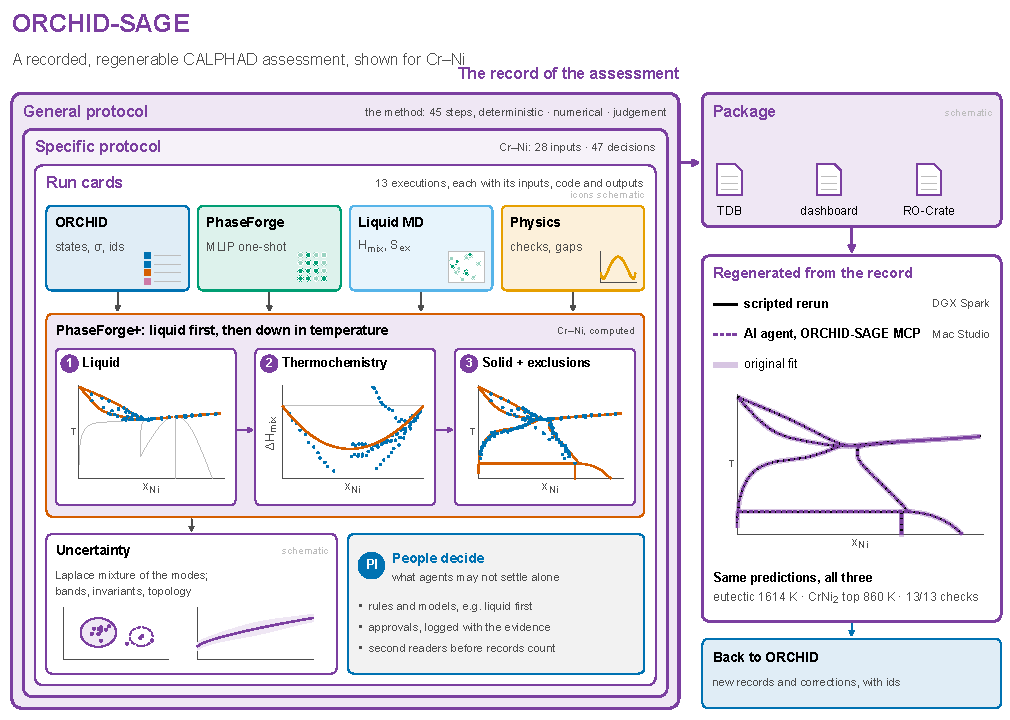
\includegraphics[width=171mm]{fig_hero}
    \caption{ORCHID-SAGE, shown for Cr--Ni. The record (general protocol, specific protocol with its decisions, run cards) wraps the assessment: ORCHID evidence, the PhaseForge one-shot model, liquid molecular dynamics, physical checks, the PhaseForge+ sequence from liquid to solid, uncertainty and the decisions made by people. The record is packaged and regenerated from itself, by a script and by an AI agent, with the same predictions. Icons are schematic. ORCHID v2026.10 and records extracted for this work; record identifiers are provided with the source data.}
    \label{fig:hero}
\end{figure*}

The CALPHAD method~\cite{lukas2007} encodes the thermodynamic properties of phases through simple, expandable models fitted to experimental and computational data. The models are then assembled into CALPHAD databases (i.e., CALPHAD model assemblages written in the standard TDB format) and fed into computational thermodynamic software~\cite{otis2017pycalphad} that, in turn, predicts a system's phase stability through constrained Gibbs free energy minimization. Over the past five decades, CALPHAD thermodynamic databases and computational thermodynamics have become central to alloy design~\cite{arroyave2022phase}. 

To date, constructing CALPHAD models remains largely labor-intensive: expert assessors collect phase equilibria and thermochemical data from the literature, select a model for each phase, and adjust model parameters until the calculated phase diagram and thermodynamic properties agree with observations~\cite{lukas2007}---in most cases, the level of agreement is assigned through subjective expert opinion. Unfortunately, many of the decisions made along the way are rarely recorded in published assessments~\cite {bocklund2019espei,arroyave2026orchid}. As a result, while publicly available CALPHAD assessments can be integrated into larger databases and then used in materials discovery and development pipelines, they are extremely difficult to regenerate from scratch or update when new data become available.

Knowing the final parameters of a model fit is not sufficient to regenerate a CALPHAD assessment from scratch. At the very minimum, we also need to know (\textbf{1}) which observations were used in the fit, preferably through links to the original measurement records; (\textbf{2}) which uncertainties were assigned; (\textbf{3}) which choices were made during the fit; and (\textbf{4}) which code, software versions, and settings were used in the process. 

In practice, however, a published thermodynamic model rarely reports more
than the final parameters resulting from the CALPHAD model fit, and most of the information needed to regenerate it is lost once the assessment is complete. The decisions of the assessor, such as the sequence of steps during the model optimization, the uncertainty attributed to each observation, the weight given to each dataset, or the choice between alternative models for a phase, are rarely written down and do not appear in the database file in which the assessment is distributed. In the end, only the authors can follow the path that led to the parameters, and even they---as the present author can attest---are \emph{usually unable to exactly reproduce their own fit after a few years}.

Of course, this problem is not unique to CALPHAD assessments. In bioinformatics, for example, data pipelines consist of long sequences of individual data analytics operations. In order to make these analyses reproducible, workflow managers such as Snakemake~\cite{molder2021snakemake} and Nextflow~\cite{ditommaso2017nextflow} and the CWL workflow language CWL~\cite{crusoe2022cwl} have become an integral part of the process. In the context of electronic-structure calculations, AiiDA records the complete provenance of every calculation~\cite{huber2020aiida} and repositories such as NOMAD~\cite{draxl2019nomad} distribute the inputs and outputs of millions of calculations. In many other computational fields, standard provenance descriptions, such as PROV-O~\cite{lebo2013provo}, and formats such as RO-Crate~\cite{soilandreyes2022rocrate,leo2024wrroc}, which bundle input, code, and output of a calculation, arose from the same need. Unfortunately, none of these practices has been adopted in CALPHAD model development, and, to the best of our knowledge, \emph{no thermodynamic database currently in use can be regenerated from what anyone---other than its authors---has published}.

\begin{figure*}[hbt]
    \centering
    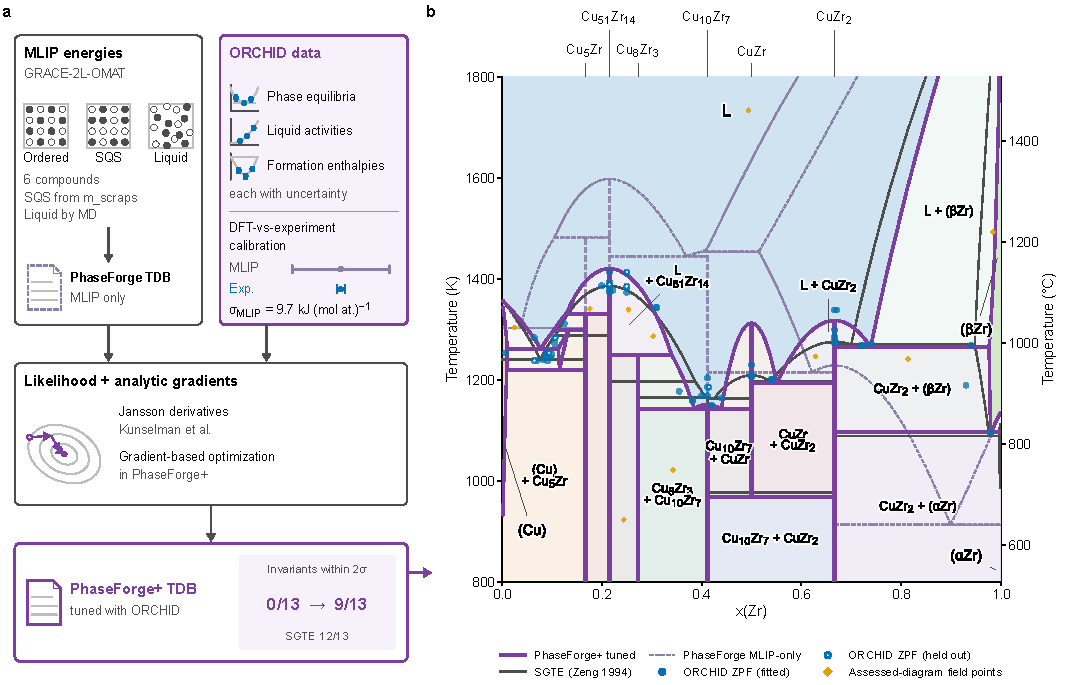
\includegraphics[width=171mm]{fig_cuzr_workflow}
    \caption{An example of an automated workflow for CALPHAD model refinement: \textbf{a}, PhaseForge constructs the starting description from MLIP compound, solid-solution and liquid energies on SGTE unary references, and PhaseForge+ combines these with uncertainty-weighted ORCHID observations using the gradient-capable ESPEI development branch. \textbf{b}, Refined diagram (violet), initial MLIP description (dashed) and SGTE assessment (grey), with fitted and held-out literature points and assessed assemblages. Reproduced, under CC BY 4.0 from ~\cite{arroyave2026orchid}.}
    \label{fig:workflow}
\end{figure*}

Since knowledge of phase stability is the first requirement for predictive synthesis, CALPHAD databases/models are expected to become increasingly important components in the toolkits available to self-driving laboratories (SDLs)~\cite{abolhasani2023selfdriving,szymanski2023alab}. In SDLs, CALPHAD-based predictions can help select synthesis/processing conditions to achieve a target phase constitution, exclude composition regions in which undesired phases form, and interpret the phases observed after synthesis. Phase stability predictions can thus help determine the next experiment to execute, and those experiments could, for example, update knowledge of phase stability if predictions are inaccurate. Updated phase stability observations could then, in principle, further refine the parameters of the CALPHAD database used to make the predictions in the first place. Within this new framework, a CALPHAD database used for predictive synthesis in this discovery loop \emph{cannot remain fixed and instead must evolve} as new evidence is acquired, enabling continuously updatable '\emph{living thermodynamic databases}'. However, this potentially transformative paradigm can only be realized if the process of developing CALPHAD assessments is automated and fully reproducible.

Machines can already perform several steps in constructing CALPHAD databases using open-source tools. \textbf{ESPEI}~\cite{bocklund2019espei}, for example, stores thermodynamic observations as machine-readable datasets that can be shared, combined and reused, and uses them to estimate both the model parameters and their uncertainty using Bayesian methods~\cite{honarmandi2019bayesian}. \textbf{ORCHID}~\cite{arroyave2026orchid}, which was built by AI agents deployed at scale over the literature, converts the reported data into thermodynamic states, each defined by its phases, temperature, pressure, and composition, with an estimate of its uncertainty and a link to the original measurement, so that the observations used in a fit can be identified one by one. The starting point of the fit, which in a manual assessment is usually a set of parameters estimated by the assessor, can in turn be computed with \textbf{PhaseForge}~\cite{zhu2025accelerating,zhu2025machinelearningpotentialsalloys}, which calculates the energies of the solution phases and compounds of an entire binary system with machine-learned interatomic potentials (MLIPs) and combines them with the SGTE descriptions of the pure elements into a first CALPHAD model. Such models reproduce the main features of many phase diagrams, but their features can be off by hundreds of kelvin, as in the Pt--W system~\cite{kunselman2025ptw}, and therefore must be refined against experimental data, a step that can be made more efficient and deterministic through advances such as gradient-based CALPHAD model optimization~\cite{kunselman2024analytically,kunselman2025analytical} as implemented in \textbf{PhaseForge+}~\cite{kunselman2025ptw,sariturk2025phaseforgeplus} (see \cref{fig:workflow}). The underlying engine of all these tools is, in turn, the \textbf{pycalphad}~\cite{otis2017pycalphad} software.

The data, the starting model, and the optimization can thus be handled by one of the tools described above. However, the assessment itself---that is, the sequence of judgments through which an expert turns these elements into a reliable database---has yet to be automated, and no existing tool records the decisions that connect its steps, which are precisely the ones left out of published assessments. An assessment obtained this way is therefore no easier to regenerate than one carried out by hand. As algorithms perform more of the CALPHAD assessment workflow, the number of these decisions increases, and most of them can no longer be examined from the resulting publications. A fully reproducible record of how a database was obtained then becomes the only way for others to verify, correct, or extend it, and the only way to carry over the expert knowledge behind an assessment to the machines meant to repeat it.

In this work, we address this problem with \textbf{ORCHID-SAGE} (\textbf{S}ystematic \textbf{A}ssessment of \textbf{G}ibbs \textbf{E}nergies), a standard for carrying out and recording CALPHAD assessments so others (including machines) can regenerate them. A sage is also ``a profoundly wise person'' and ``someone venerated for the possession of wisdom, judgment, and experience''~\cite{dictionarycom_sage}, and ORCHID-SAGE tries to capture the wisdom of the people who have made CALPHAD possible (see \textbf{Acknowledgments}). 

Our proposed standard has three levels. At the \emph{first level}, a general protocol states the rules that apply to any assessment (for example, the conversion of the uncertainty of an observation into a weight in the objective function, the phases that must be excluded at each observed state and the criterion used to choose among the solutions found from different starting points). At the \emph{second level}, a specific protocol applies these rules to one system and records the decisions made during the assessment, the reason for each, and whether a person or an algorithm made it. At the \emph{third level}, each step of the specific protocol produces a run card that identifies the inputs, code, software versions, and outputs of the step through their hashes, and then the whole evaluation is distributed as an RO-Crate~\cite{soilandreyes2022rocrate,leo2024wrroc} together with the resulting database. Since protocols can also be read by machines, an assessment can be rerun with a script or with an AI agent that uses a Model Context Protocol server~\cite{mcp}. In both cases, the new results are compared with the recorded ones within the stated tolerances. An assessment recorded this way can therefore be checked, corrected, or extended from the protocol alone, without contacting the authors.

This standard is applied here to the Cr--Ni system, which is of considerable importance to stainless steels and Ni-base superalloys and has been assessed several times~\cite{lee1992,hao2021,kunselman2026hmc}. Measurements of the solid-state phase boundaries in this system, however, remain in conflict, making it a demanding test for an assessment in which the assessor's decisions must be recorded. The assessment starts with the evidence held in ORCHID and a PhaseForge model with the SGTE descriptions of the pure elements used as reference states. This model is then refined with PhaseForge+ in a sequence that begins with the liquid and the phases that melt, where the fewest phases compete, and continues with the thermochemical and solid-state data (\cref{fig:hero}). Throughout this sequence, we weight each observation by its uncertainty rather than by hand, keep partial tie-lines as zero-phase-fraction conditions, and exclude phases stable elsewhere in the system at states where they were not observed. We also check the model's physical consistency at each stage, using, among other quantities, the excess entropy of the liquid estimated with molecular dynamics~\cite{hong2025entropy}. We then estimate the uncertainty of the final model with Laplace approximations around the posterior modes and propagate it to the phase diagram. Finally, we show that the resulting database can be regenerated using only its specific protocol, with a script on a different machine and by an AI agent, and that predictions from the rerun agree with those of the original assessment within the stated tolerances.
